\documentclass[aspectratio=43]{beamer}

% Text packages to stop warnings
\usepackage{lmodern}
\usepackage{textcomp}
\usepackage{listings}

% Themes
\usetheme{Boadilla}
\setbeamertemplate{footline}[page number]{}
\setbeamertemplate{navigation symbols}{}

% Suppress the navigation bar
\beamertemplatenavigationsymbolsempty

\lstset{basicstyle=\scriptsize, frame=single}

\newenvironment{changemargin}[1]{% 
  \begin{list}{}{% 
    \setlength{\topsep}{0pt}% 
    \setlength{\leftmargin}{#1}% 
    \setlength{\rightmargin}{1em}
    \setlength{\listparindent}{\parindent}% 
    \setlength{\itemindent}{\parindent}% 
    \setlength{\parsep}{\parskip}% 
  }% 
  \item[]}{\end{list}} 

\title{Lecture 06---A1; Race Conditions;\\ More Synchronization; Async I/O}
\date{January 21, 2014}

\begin{document}

%%%%%%%%%%%%%%%%%%%%%%%%%%%%%%%%%%%%%%%%%%%%%%%%%%%%%%%%%%%%%%%%%%%%%%%%%%%%%%%%
\begin{frame}[plain]
  \titlepage
\end{frame}
%%%%%%%%%%%%%%%%%%%%%%%%%%%%%%%%%%%%%%%%%%%%%%%%%%%%%%%%%%%%%%%%%%%%%%%%%%%%%%%%

%%%%%%%%%%%%%%%%%%%%%%%%%%%%%%%%%%%%%%%%%%%%%%%%%%%%%%%%%%%%%%%%%%%%%%%%%%%%%%%%
\begin{frame}
  \frametitle{Roadmap}

  \Large
    \begin{changemargin}{2cm}
  Past: Modern Hardware, Threads \\[1em]

  Now: A1 discussion, non-blocking I/O;\\[1em]

  Next: Race Conditions, Locking
    \end{changemargin}
  
\end{frame}
%%%%%%%%%%%%%%%%%%%%%%%%%%%%%%%%%%%%%%%%%%%%%%%%%%%%%%%%%%%%%%%%%%%%%%%%%%%%%%%%

%%%%%%%%%%%%%%%%%%%%%%%%%%%%%%%%%%%%%%%%%%%%%%%%%%%%%%%%%%%%%%%%%%%%%%%%%%%%%%%%
\begin{frame}
  \frametitle{Last Time}

  \begin{changemargin}{2.5cm}
  \begin{itemize}
    \item Processes vs threads.
    \vfill
    \item Creating, joining and exiting POSIX threads.\\
       Remember, they are 1:1 with kernel threads and can run in parallel on
      multiple CPUs.
    \vfill
    \item Difference between \structure{joinable} and \structure{detached} threads.
    \vfill
  \end{itemize}
  \end{changemargin}
\end{frame}
%%%%%%%%%%%%%%%%%%%%%%%%%%%%%%%%%%%%%%%%%%%%%%%%%%%%%%%%%%%%%%%%%%%%%%%%%%%%%%%%

\part{Assignment 1}
\frame{\partpage}

%%%%%%%%%%%%%%%%%%%%%%%%%%%%%%%%%%%%%%%%%%%%%%%%%%%%%%%%%%%%%%%%%%%%%%%%%%%%%%%%

\begin{frame}
  \frametitle{Your Task}

  \hspace*{2em} Re-assemble the picture:

  \begin{center}
  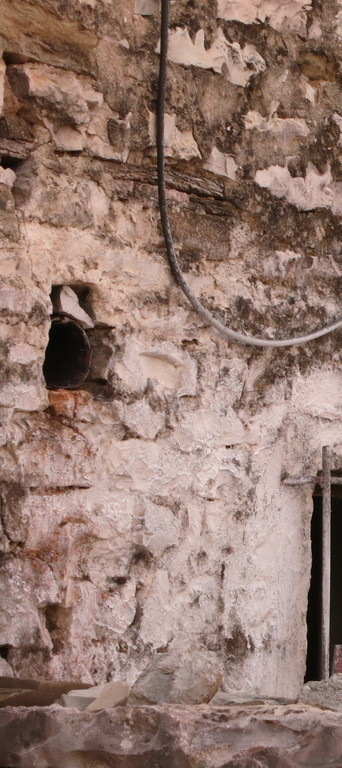
\includegraphics[width=.25\textwidth]{L06/part1} \qquad
  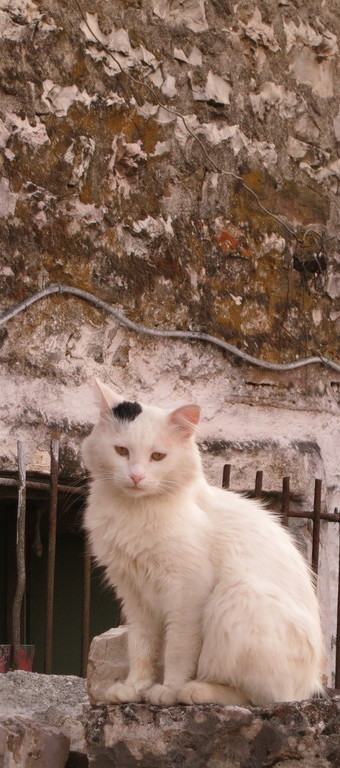
\includegraphics[width=.25\textwidth]{L06/part2} \qquad
  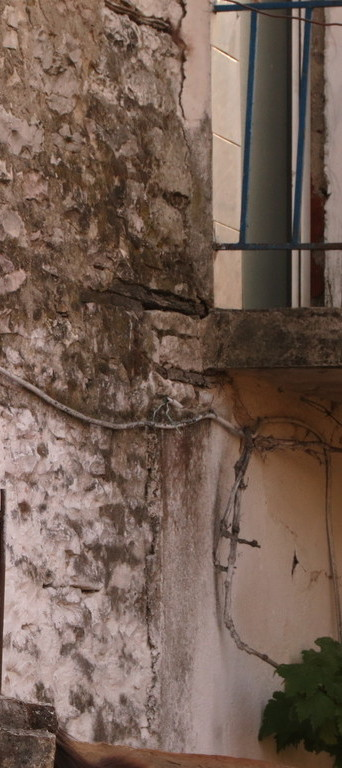
\includegraphics[width=.25\textwidth]{L06/part3}
  \end{center}
\end{frame}

%%%%%%%%%%%%%%%%%%%%%%%%%%%%%%%%%%%%%%%%%%%%%%%%%%%%%%%%%%%%%%%%%%%%%%%%%%%%%%%%

%%%%%%%%%%%%%%%%%%%%%%%%%%%%%%%%%%%%%%%%%%%%%%%%%%%%%%%%%%%%%%%%%%%%%%%%%%%%%%%%

\begin{frame}
  \frametitle{What I provide}

  \begin{changemargin}{2em}
    Serial C code:
\begin{itemize}
  \item uses curl to fetch the image over the network;
  \item uses libpng to stitch together the image.
\end{itemize}
    Plus, a web API to provide images to you.

  \end{changemargin}

\end{frame}

%%%%%%%%%%%%%%%%%%%%%%%%%%%%%%%%%%%%%%%%%%%%%%%%%%%%%%%%%%%%%%%%%%%%%%%%%%%%%%%%

%%%%%%%%%%%%%%%%%%%%%%%%%%%%%%%%%%%%%%%%%%%%%%%%%%%%%%%%%%%%%%%%%%%%%%%%%%%%%%%%
\begin{frame}
  \frametitle{What you hand in}

  \begin{changemargin}{2em}
    Part 1: pthreads parallelized implementation.\\
\begin{itemize}
  \item really easy!
  \item (also, analyze your speedups in the report.)
\end{itemize}

    Part 2: nonblocking I/O implementation.\\
\begin{itemize}
  \item more challenging;
  \item lecture today will help.
\end{itemize}

Also Parts 0, 3: analysis \& discussion.

  \end{changemargin}

\end{frame}

%%%%%%%%%%%%%%%%%%%%%%%%%%%%%%%%%%%%%%%%%%%%%%%%%%%%%%%%%%%%%%%%%%%%%%%%%%%%%%%%

%%%%%%%%%%%%%%%%%%%%%%%%%%%%%%%%%%%%%%%%%%%%%%%%%%%%%%%%%%%%%%%%%%%%%%%%%%%%%%%%
\begin{frame}
  \frametitle{Tour of the code}

  \begin{changemargin}{2em}
    main loop: while still missing some fragments,
    \begin{itemize}
      \item retrieve a fragment over the network;
      \item copy bits into our array;
    \end{itemize}
    Then, write all the bits in one PNG file.
  \end{changemargin}

\end{frame}
%%%%%%%%%%%%%%%%%%%%%%%%%%%%%%%%%%%%%%%%%%%%%%%%%%%%%%%%%%%%%%%%%%%%%%%%%%%%%%%%

%%%%%%%%%%%%%%%%%%%%%%%%%%%%%%%%%%%%%%%%%%%%%%%%%%%%%%%%%%%%%%%%%%%%%%%%%%%%%%%%
\begin{frame}[fragile]
  \frametitle{Notable bits I: retrieving the file}

  \begin{changemargin}{2em}

    Here's how I retrieve the file:

    \begin{lstlisting}
  curl_easy_setopt(curl, CURLOPT_URL, url);

  // do curl request; check for errors
  res = curl_easy_perform(curl);
    \end{lstlisting}

    But wait! I had to tell curl where to put the file:

    \begin{lstlisting}
  struct bufdata bd; 
  bd.buf = input_buffer; 
  curl_easy_setopt(curl, CURLOPT_WRITEFUNCTION, write_cb);
  curl_easy_setopt(curl, CURLOPT_WRITEDATA, &bd);
    \end{lstlisting}

    My {\tt write\_cb} callback function puts data in {\tt input\_buffer} (straightforward {\tt memcpy}-based
    implementation).

  \end{changemargin}
\end{frame}

%%%%%%%%%%%%%%%%%%%%%%%%%%%%%%%%%%%%%%%%%%%%%%%%%%%%%%%%%%%%%%%%%%%%%%%%%%%%%%%%
\begin{frame}
  \frametitle{Notable bits II: parsing the fragments}

  \begin{changemargin}{2em}

    Bunch of {\tt libpng} magic:\\

    \hspace*{1em} {\tt libpng} wants to put the image data in a {\tt png\_bytep *} array,
    where each element points to a row of pixels.\\[1em]

    My {\tt read\_png\_file} function allocates the data; caller must free.\\[1em]

    Then, {\tt paint\_destination} fills in the output array, \\pasting together
    the fragments.
  \end{changemargin}
\end{frame}
%%%%%%%%%%%%%%%%%%%%%%%%%%%%%%%%%%%%%%%%%%%%%%%%%%%%%%%%%%%%%%%%%%%%%%%%%%%%%%%%

%%%%%%%%%%%%%%%%%%%%%%%%%%%%%%%%%%%%%%%%%%%%%%%%%%%%%%%%%%%%%%%%%%%%%%%%%%%%%%%%
\begin{frame}
  \frametitle{Notable bits III: writing the output}
  \begin{changemargin}{2em}

    Well, not that notable. Symmetric to read.\\

    Note: be sure to free everything! (We'll check.)
  \end{changemargin}
\end{frame}
%%%%%%%%%%%%%%%%%%%%%%%%%%%%%%%%%%%%%%%%%%%%%%%%%%%%%%%%%%%%%%%%%%%%%%%%%%%%%%%%

%%%%%%%%%%%%%%%%%%%%%%%%%%%%%%%%%%%%%%%%%%%%%%%%%%%%%%%%%%%%%%%%%%%%%%%%%%%%%%%%
\begin{frame}
  \frametitle{Part (a): using pthreads}
  \begin{changemargin}{2em}
    You might need to refactor the code to parallelize it well.\\[1em]

    Start some threads. \\[1em] Justify why the threads are not interfering. Time the result.
  \end{changemargin}
\end{frame}

%%%%%%%%%%%%%%%%%%%%%%%%%%%%%%%%%%%%%%%%%%%%%%%%%%%%%%%%%%%%%%%%%%%%%%%%%%%%%%%%

%%%%%%%%%%%%%%%%%%%%%%%%%%%%%%%%%%%%%%%%%%%%%%%%%%%%%%%%%%%%%%%%%%%%%%%%%%%%%%%%
\begin{frame}
  \frametitle{Part (b): nonblocking I/O}
  \begin{changemargin}{2em}
    Main subject of this lecture. \\

    Will be more complicated than using threads!
  \end{changemargin}
\end{frame}

%%%%%%%%%%%%%%%%%%%%%%%%%%%%%%%%%%%%%%%%%%%%%%%%%%%%%%%%%%%%%%%%%%%%%%%%%%%%%%%%

%%%%%%%%%%%%%%%%%%%%%%%%%%%%%%%%%%%%%%%%%%%%%%%%%%%%%%%%%%%%%%%%%%%%%%%%%%%%%%%%
\begin{frame}
  \frametitle{Part (b)': JavaScript}
  \begin{changemargin}{2em}
    As an alternate option, you may use either {\tt node.js} or\\ client-side
    JavaScript to do the nonblocking I/O.\\[1em]

    Let me know if you want to do this. You are on your own, though.
  \end{changemargin}
\end{frame}
%%%%%%%%%%%%%%%%%%%%%%%%%%%%%%%%%%%%%%%%%%%%%%%%%%%%%%%%%%%%%%%%%%%%%%%%%%%%%%%%

%%%%%%%%%%%%%%%%%%%%%%%%%%%%%%%%%%%%%%%%%%%%%%%%%%%%%%%%%%%%%%%%%%%%%%%%%%%%%%%%
\part{Asynchronous/non-blocking I/O}
\frame{\partpage}
%%%%%%%%%%%%%%%%%%%%%%%%%%%%%%%%%%%%%%%%%%%%%%%%%%%%%%%%%%%%%%%%%%%%%%%%%%%%%%%%

%%%%%%%%%%%%%%%%%%%%%%%%%%%%%%%%%%%%%%%%%%%%%%%%%%%%%%%%%%%%%%%%%%%%%%%%%%%%%%%%
\begin{frame}
  \frametitle{Juicy Quotes}
  \begin{changemargin}{2em}

  \fbox{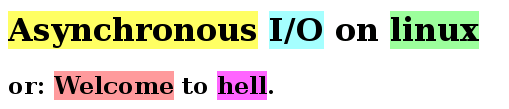
\includegraphics[width=.7\textwidth]{L06/aio-linux.png}}\\
{\scriptsize (mirrored at \url{compgeom.com/~piyush/teach/4531_06/project/hell.html})}
   \\[3em]

   ``Asynchronous I/O, for example, is often infuriating.''\\
--- Robert Love. {\em Linux System Programming, 2nd ed, } page 215.
  
  \end{changemargin}
\end{frame}
%%%%%%%%%%%%%%%%%%%%%%%%%%%%%%%%%%%%%%%%%%%%%%%%%%%%%%%%%%%%%%%%%%%%%%%%%%%%%%%%

%%%%%%%%%%%%%%%%%%%%%%%%%%%%%%%%%%%%%%%%%%%%%%%%%%%%%%%%%%%%%%%%%%%%%%%%%%%%%%%%
\begin{frame}[fragile]
  \frametitle{Why non-blocking I/O?}
  \begin{changemargin}{2em}
  Consider some I/O:

\begin{changemargin}{3em}
\begin{minipage}{.5\textwidth}
\begin{lstlisting}
    fd = open(...);
    read(...);
    close(fd);
  \end{lstlisting}
\end{minipage}
\end{changemargin}

  Not very performant---under what conditions do we lose out?
  \end{changemargin}
\end{frame}
%%%%%%%%%%%%%%%%%%%%%%%%%%%%%%%%%%%%%%%%%%%%%%%%%%%%%%%%%%%%%%%%%%%%%%%%%%%%%%%%

%%%%%%%%%%%%%%%%%%%%%%%%%%%%%%%%%%%%%%%%%%%%%%%%%%%%%%%%%%%%%%%%%%%%%%%%%%%%%%%%
\begin{frame}[fragile]
  \frametitle{Mitigating I/O impact}
  \begin{changemargin}{2em}
    So far: can use threads to mitigate latency.\\

    What are the disadvantages?
    \only<2>{
      \begin{itemize}
        \item race conditions
        \item overhead/max \# of thread limitations
      \end{itemize}
    }
  \end{changemargin}
\end{frame}
%%%%%%%%%%%%%%%%%%%%%%%%%%%%%%%%%%%%%%%%%%%%%%%%%%%%%%%%%%%%%%%%%%%%%%%%%%%%%%%%

%%%%%%%%%%%%%%%%%%%%%%%%%%%%%%%%%%%%%%%%%%%%%%%%%%%%%%%%%%%%%%%%%%%%%%%%%%%%%%%%
\begin{frame}[fragile]
  \frametitle{Live coding: forkbomb Patrick's laptop!}

\begin{center}
(well, threadbomb anyway)
\end{center}

\end{frame}
%%%%%%%%%%%%%%%%%%%%%%%%%%%%%%%%%%%%%%%%%%%%%%%%%%%%%%%%%%%%%%%%%%%%%%%%%%%%%%%%

%%%%%%%%%%%%%%%%%%%%%%%%%%%%%%%%%%%%%%%%%%%%%%%%%%%%%%%%%%%%%%%%%%%%%%%%%%%%%%%%
\begin{frame}[fragile]
  \frametitle{An Alternative to Threads}
  \begin{changemargin}{2em}
    Asynchronous/nonblocking I/O.\\[2em]

\begin{changemargin}{3em}
\begin{minipage}{.6\textwidth}
\begin{lstlisting}
    fd = open(..., O_NONBLOCK);
    read(...); // returns instantly!
    close(fd);
  \end{lstlisting}
\end{minipage}
\end{changemargin}

\begin{center}
~\\[1em]
$\cdots$\\[2em]


\includegraphics[width=.25\textwidth]{L06/Easy_button.JPG}
\end{center}
\hfill {\scriptsize (credit: Yskyflyer, Wikimedia Commons)}

  \end{changemargin}
\end{frame}
%%%%%%%%%%%%%%%%%%%%%%%%%%%%%%%%%%%%%%%%%%%%%%%%%%%%%%%%%%%%%%%%%%%%%%%%%%%%%%%%

%%%%%%%%%%%%%%%%%%%%%%%%%%%%%%%%%%%%%%%%%%%%%%%%%%%%%%%%%%%%%%%%%%%%%%%%%%%%%%%%
\begin{frame}
  \frametitle{Not Quite So Easy: Live Demo}
  \begin{changemargin}{2em}
    Doesn't work on files---they're always ready. Only e.g. sockets.
  \end{changemargin}
\end{frame}
%%%%%%%%%%%%%%%%%%%%%%%%%%%%%%%%%%%%%%%%%%%%%%%%%%%%%%%%%%%%%%%%%%%%%%%%%%%%%%%%

%%%%%%%%%%%%%%%%%%%%%%%%%%%%%%%%%%%%%%%%%%%%%%%%%%%%%%%%%%%%%%%%%%%%%%%%%%%%%%%%
\begin{frame}
  \frametitle{Other Outstanding Problem with Nonblocking I/O}
  \begin{changemargin}{2em}
    How do you know when I/O is ready to be queried?

    \only<2>{\begin{itemize} 
      \item polling ({\tt select}, {\tt poll}, {\tt epoll})
      \item interrupts (signals)
      \end{itemize}
    }
  \end{changemargin}
\end{frame}
%%%%%%%%%%%%%%%%%%%%%%%%%%%%%%%%%%%%%%%%%%%%%%%%%%%%%%%%%%%%%%%%%%%%%%%%%%%%%%%%

%%%%%%%%%%%%%%%%%%%%%%%%%%%%%%%%%%%%%%%%%%%%%%%%%%%%%%%%%%%%%%%%%%%%%%%%%%%%%%%%
\begin{frame}
  \frametitle{Using {\tt epoll}}
  \begin{changemargin}{2em}
    Key idea: give {\tt epoll} a bunch of file descriptors;\\
     \hspace*{2em}wait for events to happen.\\[1em]

     Steps:
     \begin{enumerate}
       \item create an instance ({\tt epoll\_create1});
       \item populate it with file descriptors ({\tt epoll\_ctl});
       \item wait for events ({\tt epoll\_wait}).
     \end{enumerate}
  \end{changemargin}
\end{frame}
%%%%%%%%%%%%%%%%%%%%%%%%%%%%%%%%%%%%%%%%%%%%%%%%%%%%%%%%%%%%%%%%%%%%%%%%%%%%%%%%

%%%%%%%%%%%%%%%%%%%%%%%%%%%%%%%%%%%%%%%%%%%%%%%%%%%%%%%%%%%%%%%%%%%%%%%%%%%%%%%%
\begin{frame}[fragile]
  \frametitle{Creating an {\tt epoll} instance}
  \begin{changemargin}{2em}
    \begin{minipage}{.5\textwidth}
    \begin{lstlisting}
   int epfd = epoll_create1(0);
    \end{lstlisting}
    \end{minipage}

    {\tt efpd} doesn't represent any files; use it to talk to {\tt epoll}.\\[1em]

    0 represents the flags (only flag: {\tt EPOLL\_CLOEXEC}).
    
  \end{changemargin}
\end{frame}
%%%%%%%%%%%%%%%%%%%%%%%%%%%%%%%%%%%%%%%%%%%%%%%%%%%%%%%%%%%%%%%%%%%%%%%%%%%%%%%%

%%%%%%%%%%%%%%%%%%%%%%%%%%%%%%%%%%%%%%%%%%%%%%%%%%%%%%%%%%%%%%%%%%%%%%%%%%%%%%%%
\begin{frame}[fragile]
  \frametitle{Populating the {\tt epoll} instance}
  \begin{changemargin}{2em}
    To add {\tt fd} to the set of descriptors watched by {\tt epfd}:
    \begin{lstlisting}
   struct epoll_event event;
   int ret;
   event.data.fd = fd;
   event.events = EPOLLIN | EPOLLOUT;
   ret = epoll_ctl(epfd, EPOLL_CTL_ADD, fd, &event);
    \end{lstlisting}

    Can also modify and delete descriptors from {\tt epfd}.
  \end{changemargin}
\end{frame}
%%%%%%%%%%%%%%%%%%%%%%%%%%%%%%%%%%%%%%%%%%%%%%%%%%%%%%%%%%%%%%%%%%%%%%%%%%%%%%%%

%%%%%%%%%%%%%%%%%%%%%%%%%%%%%%%%%%%%%%%%%%%%%%%%%%%%%%%%%%%%%%%%%%%%%%%%%%%%%%%%
\begin{frame}[fragile]
  \frametitle{Waiting on an {\tt epoll} instance}
  \begin{changemargin}{2em}
    Now we're ready to wait for events on any file descriptor in {\tt epfd}.
    \begin{lstlisting}
  #define MAX_EVENTS 64

  struct epoll_event events[MAX_EVENTS];
  int nr_events;

  nr_events = epoll_wait(epfd, events, MAX_EVENTS, -1);
    \end{lstlisting}

-1: wait potentially forever; otherwise, milliseconds to wait.\\[1em]

Upon return from {\tt epoll\_wait}, we have {\tt nr\_events} events ready.

  \end{changemargin}
\end{frame}
%%%%%%%%%%%%%%%%%%%%%%%%%%%%%%%%%%%%%%%%%%%%%%%%%%%%%%%%%%%%%%%%%%%%%%%%%%%%%%%%

%%%%%%%%%%%%%%%%%%%%%%%%%%%%%%%%%%%%%%%%%%%%%%%%%%%%%%%%%%%%%%%%%%%%%%%%%%%%%%%%
\begin{frame}
  \frametitle{Level-Triggered and Edge-Triggered Events}
  \begin{changemargin}{2em}
    Default {\tt epoll} behaviour is \structure{level-triggered}:\\
    \quad return whenever data is ready.\\[1em]

    Can also specify (via {\tt epoll\_ctl}) \structure{edge-triggered} behaviour:\\
    \quad return whenever there is a change in readiness.\\[1em]

    We'll see an example next time.

  \end{changemargin}
\end{frame}
%%%%%%%%%%%%%%%%%%%%%%%%%%%%%%%%%%%%%%%%%%%%%%%%%%%%%%%%%%%%%%%%%%%%%%%%%%%%%%%%

%%%%%%%%%%%%%%%%%%%%%%%%%%%%%%%%%%%%%%%%%%%%%%%%%%%%%%%%%%%%%%%%%%%%%%%%%%%%%%%%
\begin{frame}
  \frametitle{Asynchronous I/O}
  \begin{changemargin}{2em}
    POSIX standard defines \structure{aio} calls.\\[1em]

    These work for disk as well as sockets.\\[1em]

    Key idea: you specify the action to occur when I/O is ready:
    \begin{itemize}
      \item nothing;
      \item start a new thread;
      \item raise a signal
    \end{itemize}

    Submit the requests using e.g. {\tt aio\_read} and {\tt aio\_write}.\\[1em]
    Can wait for I/O to happen using {\tt aio\_suspend}.
  \end{changemargin}
\end{frame}
%%%%%%%%%%%%%%%%%%%%%%%%%%%%%%%%%%%%%%%%%%%%%%%%%%%%%%%%%%%%%%%%%%%%%%%%%%%%%%%%

%%%%%%%%%%%%%%%%%%%%%%%%%%%%%%%%%%%%%%%%%%%%%%%%%%%%%%%%%%%%%%%%%%%%%%%%%%%%%%%%
\begin{frame}
  \frametitle{Nonblocking I/O with curl}
  \begin{changemargin}{2em}
    Similar idea to {\tt epoll}:
\begin{itemize}
\item build up a set of descriptors;
\item invoke the transfers and wait for them to finish;
\item see how things went.
\end{itemize}
  \end{changemargin}
\end{frame}
%%%%%%%%%%%%%%%%%%%%%%%%%%%%%%%%%%%%%%%%%%%%%%%%%%%%%%%%%%%%%%%%%%%%%%%%%%%%%%%%


%%%%%%%%%%%%%%%%%%%%%%%%%%%%%%%%%%%%%%%%%%%%%%%%%%%%%%%%%%%%%%%%%%%%%%%%%%%%%%%%
\part{Race Conditions}
\frame{\partpage}
%%%%%%%%%%%%%%%%%%%%%%%%%%%%%%%%%%%%%%%%%%%%%%%%%%%%%%%%%%%%%%%%%%%%%%%%%%%%%%%%

%%%%%%%%%%%%%%%%%%%%%%%%%%%%%%%%%%%%%%%%%%%%%%%%%%%%%%%%%%%%%%%%%%%%%%%%%%%%%%%%
\begin{frame}
  \frametitle{Race Conditions}

  \begin{changemargin}{2.5cm}
  \begin{itemize}
    \item A race occurs when you have two concurrent accesses to the
      same memory location, at least one of which is a {\bf write}.
  \end{itemize}~\\

   When there's a race, the final state may not be the same as
      running one access to completion and then the other.\\[1em]
   Race conditions arise between variables which
      are shared between threads.
  \end{changemargin}

\end{frame}
%%%%%%%%%%%%%%%%%%%%%%%%%%%%%%%%%%%%%%%%%%%%%%%%%%%%%%%%%%%%%%%%%%%%%%%%%%%%%%%%

%%%%%%%%%%%%%%%%%%%%%%%%%%%%%%%%%%%%%%%%%%%%%%%%%%%%%%%%%%%%%%%%%%%%%%%%%%%%%%%%
\begin{frame}[fragile]
  \frametitle{Example Data Race (Part 1)}

  \begin{changemargin}{2.5cm}
  \begin{lstlisting}
#include <stdlib.h>
#include <stdio.h>
#include <pthread.h>

void* run1(void* arg)
{
    int* x = (int*) arg;
    *x += 1;
}

void* run2(void* arg)
{
    int* x = (int*) arg;
    *x += 2;
}
  \end{lstlisting}
\end{changemargin}
\end{frame}
%%%%%%%%%%%%%%%%%%%%%%%%%%%%%%%%%%%%%%%%%%%%%%%%%%%%%%%%%%%%%%%%%%%%%%%%%%%%%%%%

%%%%%%%%%%%%%%%%%%%%%%%%%%%%%%%%%%%%%%%%%%%%%%%%%%%%%%%%%%%%%%%%%%%%%%%%%%%%%%%%
\begin{frame}[fragile]
  \frametitle{Example Data Race (Part 2)}

  \begin{changemargin}{2.5cm}
  \begin{lstlisting}
int main(int argc, char *argv[])
{
    int* x = malloc(sizeof(int));
    *x = 1;
    pthread_t t1, t2;
    pthread_create(&t1, NULL, &run1, x);
    pthread_join(t1, NULL);
    pthread_create(&t2, NULL, &run2, x);
    pthread_join(t2, NULL);
    printf("%d\n", *x);
    free(x);
    return EXIT_SUCCESS;
}
  \end{lstlisting}

     Do we have a data race? Why or why not?
  
  \begin{itemize}
    \item<2-> No, we don't. Only one thread is active at a time.
  \end{itemize}
   \end{changemargin}


\end{frame}
%%%%%%%%%%%%%%%%%%%%%%%%%%%%%%%%%%%%%%%%%%%%%%%%%%%%%%%%%%%%%%%%%%%%%%%%%%%%%%%%

%%%%%%%%%%%%%%%%%%%%%%%%%%%%%%%%%%%%%%%%%%%%%%%%%%%%%%%%%%%%%%%%%%%%%%%%%%%%%%%%
\begin{frame}[fragile]
  \frametitle{Example Data Race (Part 2B)}

  \begin{changemargin}{2.5cm}
  \begin{lstlisting}
int main(int argc, char *argv[])
{
    int* x = malloc(sizeof(int));
    *x = 1;
    pthread_t t1, t2;
    pthread_create(&t1, NULL, &run1, x);
    pthread_create(&t2, NULL, &run2, x);
    pthread_join(t1, NULL);
    pthread_join(t2, NULL);
    printf("%d\n", *x);
    free(x);
    return EXIT_SUCCESS;
}
  \end{lstlisting}

    Do we have a data race now? Why or why not?
  \begin{itemize}
    \item <2-> Yes, we do. We have 2 threads concurrently accessing the same data.
  \end{itemize}
   \end{changemargin}

\end{frame}
%%%%%%%%%%%%%%%%%%%%%%%%%%%%%%%%%%%%%%%%%%%%%%%%%%%%%%%%%%%%%%%%%%%%%%%%%%%%%%%%

%%%%%%%%%%%%%%%%%%%%%%%%%%%%%%%%%%%%%%%%%%%%%%%%%%%%%%%%%%%%%%%%%%%%%%%%%%%%%%%%
\begin{frame}[fragile]
  \frametitle{Tracing our Example Data Race}

  \begin{changemargin}{2.5cm}
   What are the possible outputs? (initially {\tt *x} is 1).

  \begin{lstlisting}[numbers=left]
run1                          run2   
D.1 = *x;                     D.1 = *x;
D.2 = D.1 + 1;                D.2 = D.1 + 2
*x = D.2;                     *x = D.2;
  \end{lstlisting}

  \begin{itemize}
    \item Memory reads and writes are key in data~races.
  \end{itemize}
  \end{changemargin}

\end{frame}
%%%%%%%%%%%%%%%%%%%%%%%%%%%%%%%%%%%%%%%%%%%%%%%%%%%%%%%%%%%%%%%%%%%%%%%%%%%%%%%%

%%%%%%%%%%%%%%%%%%%%%%%%%%%%%%%%%%%%%%%%%%%%%%%%%%%%%%%%%%%%%%%%%%%%%%%%%%%%%%%%
\begin{frame}
  \frametitle{Outcome of Example Data Race}

  \begin{changemargin}{2cm}
  \begin{itemize}
    \item Let's call the read and write from {\tt run1} R1 and W1; R2 and W2
      from {\tt run2}.
    \item Assuming a sane\footnote{sequentially consistent} memory model, $R_n$ must precede $W_n$.
  \end{itemize}
  \vfill
  All possible orderings:
  \begin{center}
    \begin{tabular}{llll|l}
\multicolumn{4}{c|}{Order} & {\tt *x}\\
\hline
R1 & W1 & R2 & W2 & 4 \\
R1 & R2 & W1 & W2 & 3 \\
R1 & R2 & W2 & W1 & 2 \\
R2 & W2 & R1 & W1 & 4 \\
R2 & R1 & W2 & W1 & 2 \\
R2 & R1 & W1 & W2 & 3 \\
    \end{tabular}
  \end{center}
  \end{changemargin}

\end{frame}
%%%%%%%%%%%%%%%%%%%%%%%%%%%%%%%%%%%%%%%%%%%%%%%%%%%%%%%%%%%%%%%%%%%%%%%%%%%%%%%%

%%%%%%%%%%%%%%%%%%%%%%%%%%%%%%%%%%%%%%%%%%%%%%%%%%%%%%%%%%%%%%%%%%%%%%%%%%%%%%%%
\begin{frame}
  \frametitle{Detecting Data Races Automatically}  

  \begin{changemargin}{2.5cm}
    Dynamic and static tools can help find data races in your program.
  \begin{itemize}
    \item {\tt helgrind} is one such tool. It runs your program 
      and analyzes it (and causes a large slowdown).
  \end{itemize}
    Run with {\tt valgrind --tool=helgrind <prog>}.\\[1em]
    It will warn you of possible data races along with locations.\\[1em]
    For useful debugging information, compile with debugging information
      ({\tt -g} flag for {\tt gcc}).
  \end{changemargin}
\end{frame}
%%%%%%%%%%%%%%%%%%%%%%%%%%%%%%%%%%%%%%%%%%%%%%%%%%%%%%%%%%%%%%%%%%%%%%%%%%%%%%%%

%%%%%%%%%%%%%%%%%%%%%%%%%%%%%%%%%%%%%%%%%%%%%%%%%%%%%%%%%%%%%%%%%%%%%%%%%%%%%%%%
\begin{frame}[fragile]
  \frametitle{Helgrind Output for Example}

  \begin{changemargin}{.8cm}
  \begin{lstlisting}
==5036== Possible data race during read of size 4 at
         0x53F2040 by thread #3
==5036== Locks held: none
==5036==    at 0x400710: run2 (in datarace.c:14)
...
==5036== 
==5036== This conflicts with a previous write of size 4 by
         thread #2
==5036== Locks held: none
==5036==    at 0x400700: run1 (in datarace.c:8)
...
==5036== 
==5036== Address 0x53F2040 is 0 bytes inside a block of size
         4 alloc'd
...
==5036==    by 0x4005AE: main (in datarace.c:19)
  \end{lstlisting}
  \end{changemargin}
\end{frame}
%%%%%%%%%%%%%%%%%%%%%%%%%%%%%%%%%%%%%%%%%%%%%%%%%%%%%%%%%%%%%%%%%%%%%%%%%%%%%%%%
\end{document}
